% Chapter Template

\chapter{Project Objectives} % Main chapter title

\label{Chapter1} % Change X to a consecutive number; for referencing this chapter elsewhere, use \cref{ChapterX}

%----------------------------------------------------------------------------------------
%	SECTION 1
%----------------------------------------------------------------------------------------


For this project, a JassBot is created and trained to play against itself.
For this purpose, a reinforcement learning algorithm will be trained to find the best game strategy.
The baseline will be the random pick of a playable card for comparison.\\

\section{Deck \cite{jass}}
Jass is played with a deck of 36 cards (Ace, King, Queen, Jack, 10, 9, 8, 7, 6) Swiss-French or Swiss-German cards (Ass, König, Ober, Under, Banner (= 10), 9, 8, 7, 6). The Swiss-German cards use Swiss suits, a variant of German suits, and have a distinctive design.\\


The game is traditionally played with Swiss-suited cards east of the Brünig-Napf-Reuss line \cite{reuss} and with French cards in western Switzerland. \\
The Swiss suits are Rosen (roses), Eicheln (acorns), Schellen (bells), and Schilten (shields)
\begin{figure}[ht!]
    \centering
    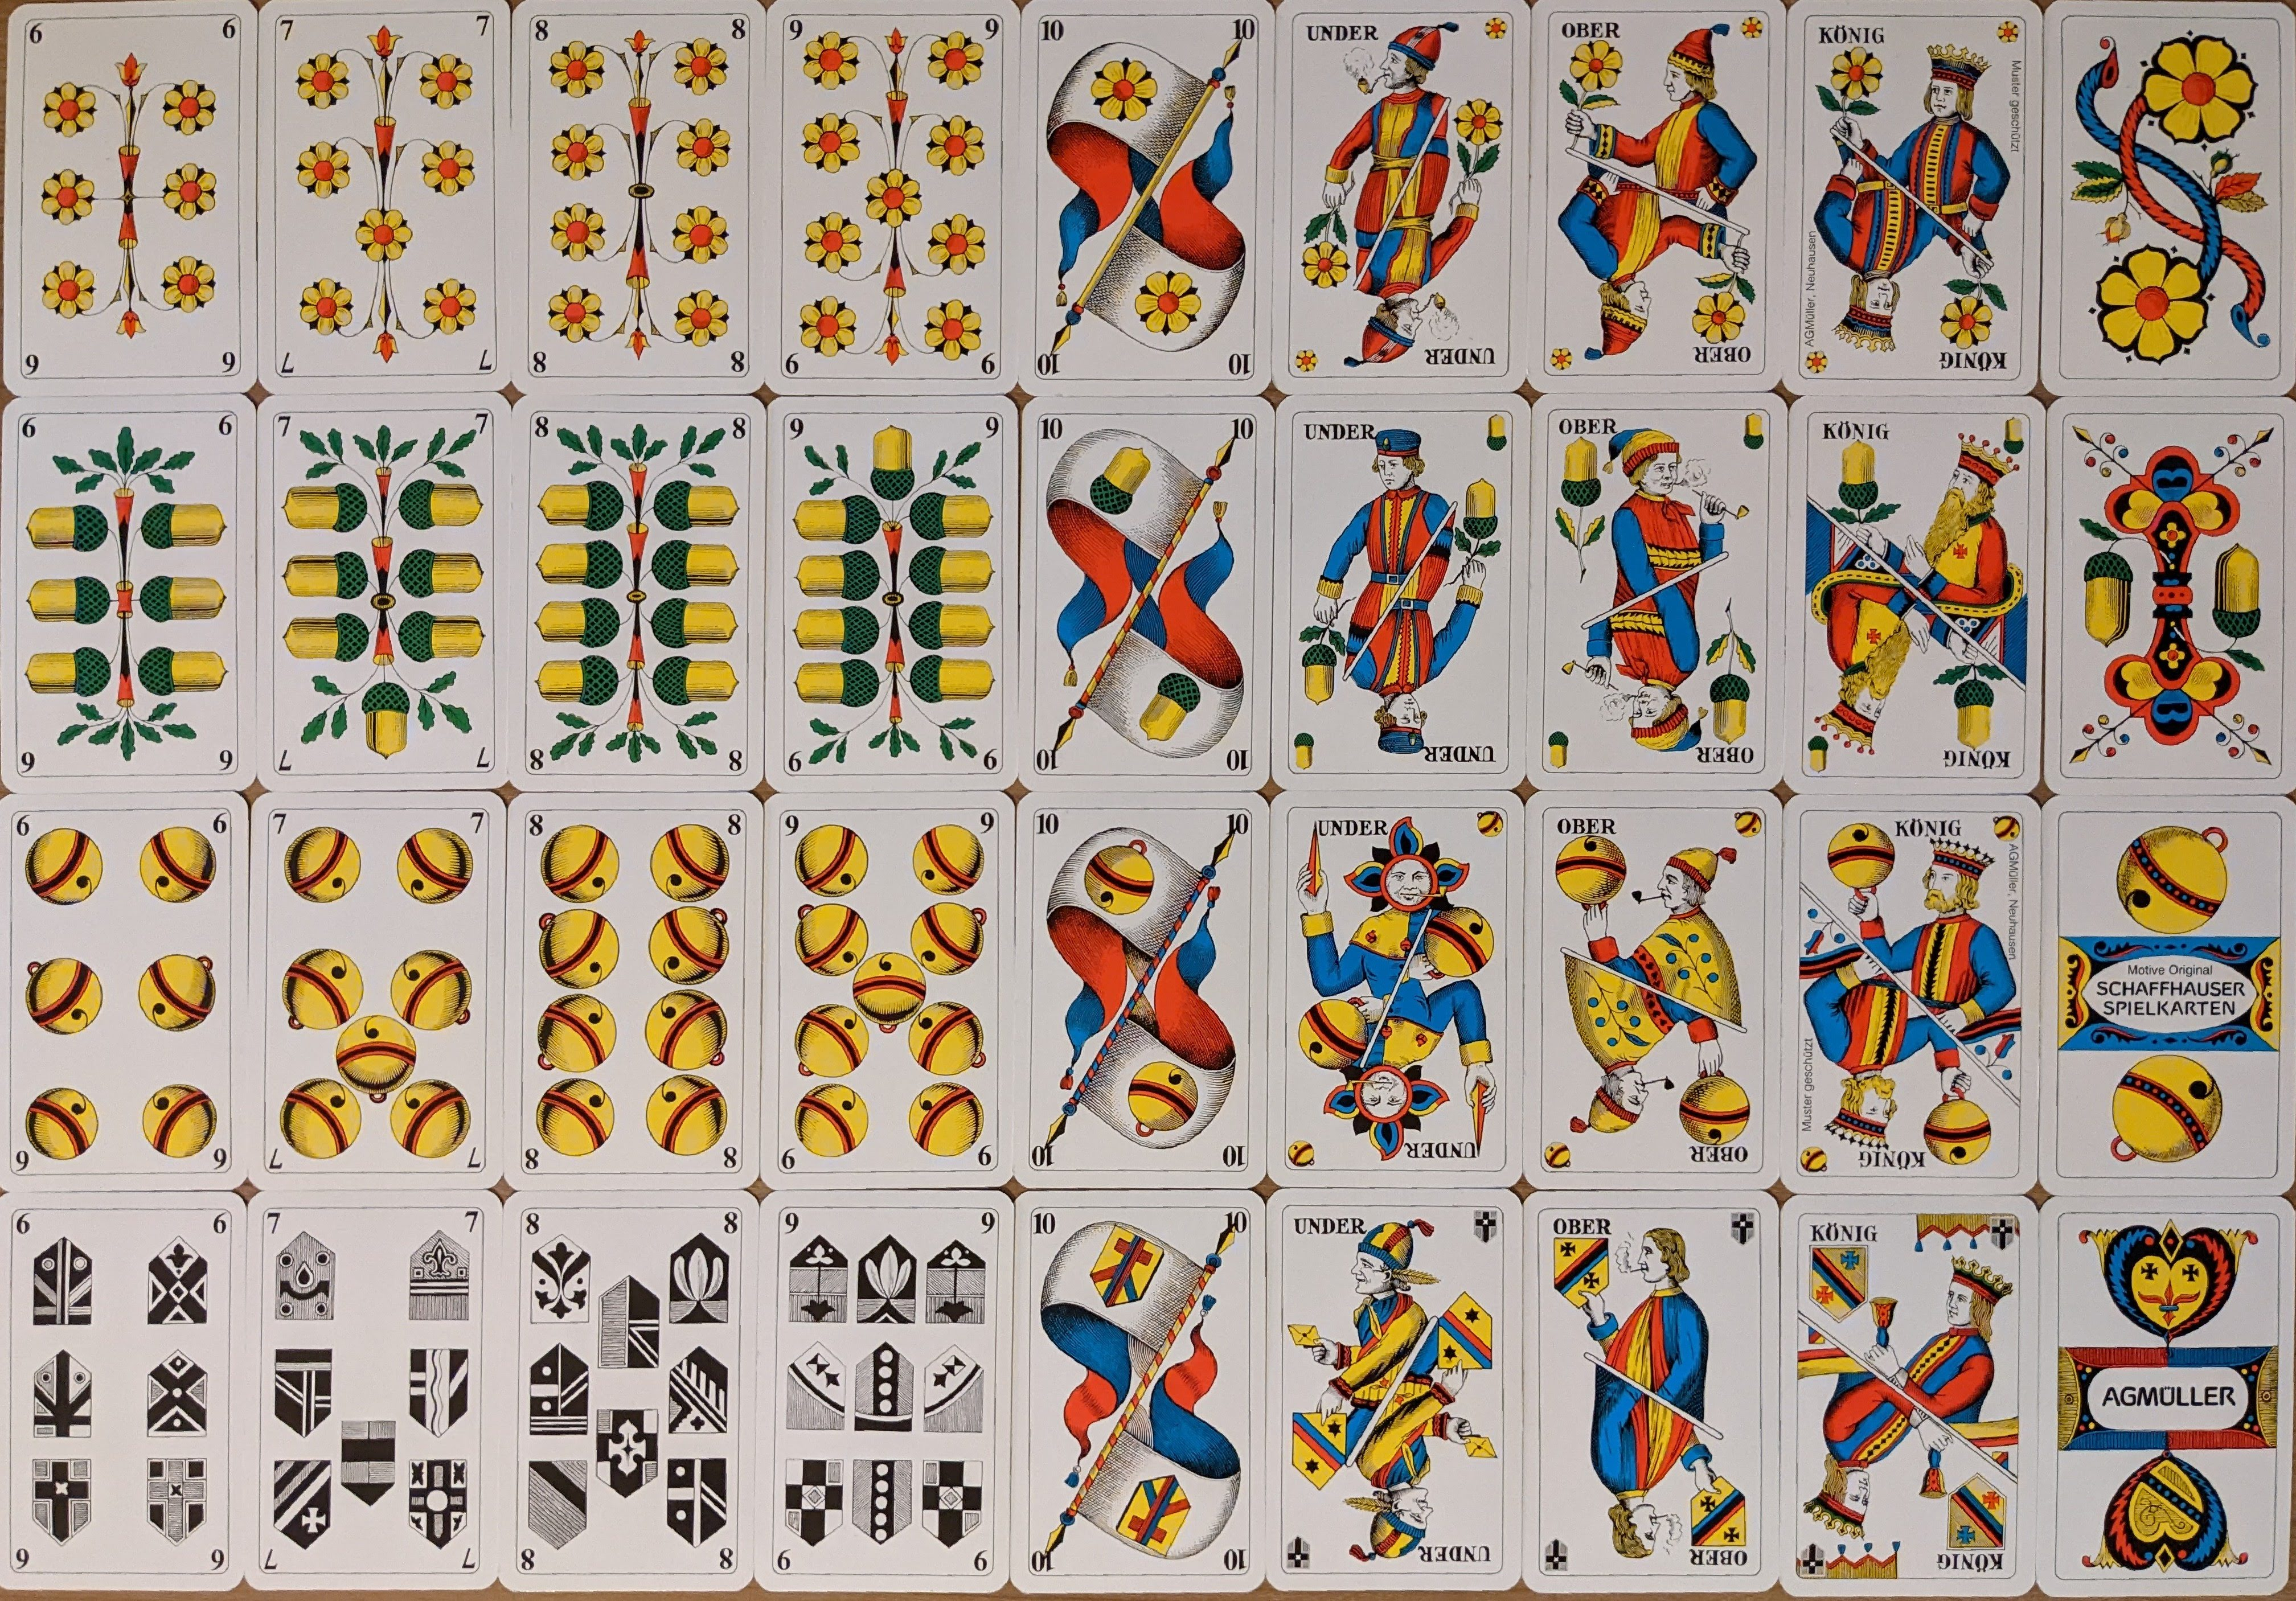
\includegraphics[width=1.0\textwidth]{Figures/jasskarten_de_ch}
    \decoRule
    \caption[Swiss German Cards]{Swiss German Cards}
    \label{fig:SwissGermanCards}
\end{figure}



\section{Game variants}
Jassen is the collective term for different game variants with different numbers of players. In most variants, each player receives nine cards (hand).
The most popular variant is the Schieber, where two teams of 2 players play against each other until one team reaches the points needed to win.
Another well-known game variant is the Differenzler (known from the TV show Samstagsjass). Here four players play against each other; before each deal, each player announces how many points he intends to make in this round. The difference to the actual score is noted as penalty points and added at each round. The player with the least penalty points wins.
Another game variant is the Handjass, which can be played in pairs, threes, or fours. In each round, the player who takes the most points scores a stroke, and anyone who takes fewer than 26 points gets a Null - sometimes known as a Herdöpfel (potato) - which is worth minus one stroke. The player who achieves a net score of 7 strokes wins and retires from the game: the loser is the last player who fails to reach seven strokes. \cite{handjass}\\

\section{Rules \cite{jass}}
Jass is a game of points scored for three features: Stöck, Wiis, and Stich, respectively, "marriages, melds, tricks.


\subsection{Tricks}

The trump Jack, also called Puur, counts 20 and is the highest card in the game. The trump Nine, or Nell, Näll, is the second-best card. Plain suit numerals below 10 count nothing. The total value of all counters in the pack is 152, that is, 62 in trumps plus 30 in each plain suit. Winning the last trick scores an additional 5 points. Hence the total possible for the third scoring feature, "tricks," usually is 157 points.

The rank of the cards, from highest to lowest, and their values in card points are shown in the following table:

\begin{table}[ht!]
    \caption{Card Values - trump games}
    \label{tab:Card Values - trump games}
    \begin{center}
        \begin{tabular}{|l|c|c|c|c|c|c|c|c|c|c|c|}
             \hline
             \multicolumn{12}{|c|}{\textbf{Card Values}} \\ \hline
             Plain suit rank & & & A & K & O/Q & U/J & 10 & 9 & 8 & 7 & 6 \\ \hline
             Value & 20 &  14 & 11 & 4 & 3 &   & 10 &   & 0 & 0 & 0 \\ \hline
             Trump suit rank & J/U & 9 & A & K & O/Q & U/J & 10 & 9 & 8 & 7 & 6 \\ \hline
        \end{tabular}
    \end{center}
\end{table}

The no-trumps game called Obenabe and Undenufe, in which the ranks are reversed, are shown in the following table:
\begin{table}[ht!]
    \caption{Card Values - no-trump games}
    \label{tab:Card Values - no-trump games}
    \begin{center}
        \begin{tabular}{|l|c|c|c|c|c|c|c|c|c||c|c|c|c|c|c|c|c|c|}
             \hline
             \multicolumn{19}{|c|}{\textbf{Card Values}} \\ \hline
             \multicolumn{10}{|c||}{Obenabe} & \multicolumn{9}{c|}{Undenufe} \\ \hline
             Rank & A & K & O/Q & U/J & 10 & 9 & 8 & 7 & 6 & 6 & 7 & 8 & 9 & 10 & U/J & O/Q & K & A  \\ \hline
             Value & 11 & 4 & 3 & 2 & 10 & 0 & 8 & 0 & 0 & 11 & 0 & 8 & 0 & 10 & 2 & 3 & 4 & 0 \\ \hline
        \end{tabular}
    \end{center}
\end{table}


\subsection{Marriage}
Marriage (Stöck): A marriage is the holding in one hand of the König and Ober (King and Queen) of trump. Its holder claims it upon the second of them to a trick. Its score of 20 is recorded as if made before those for melds and tricks, even though it is not revealed until after melds have been declared.

\subsection{Melds}
Meld (Wys or Weis): A meld is a suit sequence of three or more cards or a quartet of Aces, Kings, Queens, or Jacks scoring as follows:
    
\begin{itemize}
    \item Four Jacks: scores 200
    \item Four 9's: scores 150
    \item Five or more in suit sequence: scores 100
    \item Four A, K, Q, 10: scores 100
    \item Four in suit sequence: scores 50
    \item Three in suit sequence: scores 20
\end{itemize} 
        
A card may not be used in two melds at once, though the trump King or Queen may belong to a meld in addition to being married; that is, a player holding four Kings and a sequence of four to the Ace or King would count only 100 for Kings, not also 50 for the sequence.



\section{Chosen Game and Rules for this Project}
For this project, a two-player Handjass was used, hoping to minimize the game's complexity. It was also decided not to use Marriage and Melds, as these scores are obtained randomly and do not contribute to learning a game strategy. A further decision was not to implement the five scores for the last-round winner to minimize the programming effort.
If this project finds a successful game strategy, the remaining game elements can be added in a later version.\\






